\documentclass[a4paper]{report}

%====================== PACKAGES ======================

\usepackage[french]{babel}
\usepackage[utf8x]{inputenc}
\usepackage{float}
\usepackage{amsmath}
\usepackage{xr}
\usepackage{graphicx}
\usepackage[colorinlistoftodos]{todonotes}
\usepackage{url}
\usepackage[colorlinks=true,urlcolor=blue]{hyperref}
\usepackage{array}
\usepackage{tabularx}
\usepackage{setspace}
\usepackage{abstract}
\usepackage[T1]{fontenc}
\usepackage[top=2cm, bottom=2cm, left=2cm, right=2cm]{geometry}
\usepackage{subfig}
\usepackage{multirow}
\usepackage{listings}
\usepackage{color}
\usepackage{hhline}
\definecolor{deepblue}{rgb}{0,0,0.5}
\definecolor{deepred}{rgb}{0.6,0,0}
\definecolor{deepgreen}{rgb}{0,0.5,0}
\usepackage{listings}
\usepackage{url}
\lstdefinestyle{numbers} {numbers=left, stepnumer=1, numberstyle=\tiny, numbersep=10pt}
\lstdefinestyle{MyFrame}{backgroundcolor=\color{white},frame=shadowbox}
\lstdefinestyle{MyBashStyle}{language=bash,style=numbers,style=MyFrame,frames=lines}
\lstdefinestyle{MyPythonStyle}{language=python,style=numbers,style=MyFrame,frame=lines}
\lstset{language=bash,frame=lines}
\lstset{language=python,frame=lines}

\newcommand\pythonstyle{\lstset{
language=Python,
style=numbers,
basicstyle=\ttfamily\scriptsize,
otherkeywords={self},{True},{False},             % Add keywords here
keywordstyle=\color{deepblue}\bfseries,
commentstyle=\color{deepred},
stringstyle=\color{deepgreen},
showstringspaces=false
frame=tb,
showstringspaces=false
}}

\newcommand\pythonexternal[2][]{{
\pythonstyle
\lstinputlisting[#1]{#2}}}


%====================== INFORMATION ET REGLES ======================

\setcounter{secnumdepth}{4}
\setcounter{tocdepth}{4}
\hypersetup{			
pdfauthor = {Florian GRANTE},	
pdftitle = {FABLAB : Atelier de découverte Arduino N°1},
pdfsubject = {Atelier 1},
pdfkeywords = {Arduino, Fablab, TSP, TEM, TMSP},
pdfstartview={FitH}}
%======================== DEBUT DU DOCUMENT ========================
\begin{document}
\newcommand{\HRule}{\rule{\linewidth}{0.5mm}}
\begin{titlepage}
\begin{center}

% Upper part of the page. The '~' is needed because only works if a paragraph has started.

\includegraphics[width=0.8\textwidth]{./images/tsp}~\\[1cm]

\textsc{\LARGE Atelier de formation FabLab : Arduino}\\[1.5cm]

\textsc{\Large }\\[0.5cm]

% Title
\HRule \\[0.4cm]

{\huge \bfseries Atelier 1 : Découverte de Arduino\\[0.4cm] }

\HRule \\[1.5cm]

% Author and supervisor
\begin{minipage}{0.4\textwidth}
\begin{flushleft} \large
\emph{Auteur:}\\
Florian \textsc{GRANTE}\\
\end{flushleft}
\end{minipage}
\begin{minipage}{0.4\textwidth}
\begin{flushright} \large
\emph{Relecture:} \\
Rémi \textsc{DULONG}
\end{flushright}
\end{minipage}

\vfill

% Bottom of the page
{\large \today}

\end{center}
\end{titlepage}
\thispagestyle{empty}
\tableofcontents
\thispagestyle{empty}
\setcounter{page}{0}
\renewcommand{\arraystretch}{1.5}
%====================== INCLUSION DES PARTIES ======================
~
\thispagestyle{empty}
\setcounter{page}{0}
\newpage
\chapter*{Fiche pratique}

\addcontentsline{toc}{chapter}{Fiche pratique}

\section{Déroulement :}\\

\begin{itemize}\\
	\item Présentation succinte de la carte Arduino et des éléments de base du kit (BreakBoard, fils d'interconnexion, LEDs, capteurs,...)\\
\begin{figure}[H]
	\begin{center}
		\makebox[\textwidth]{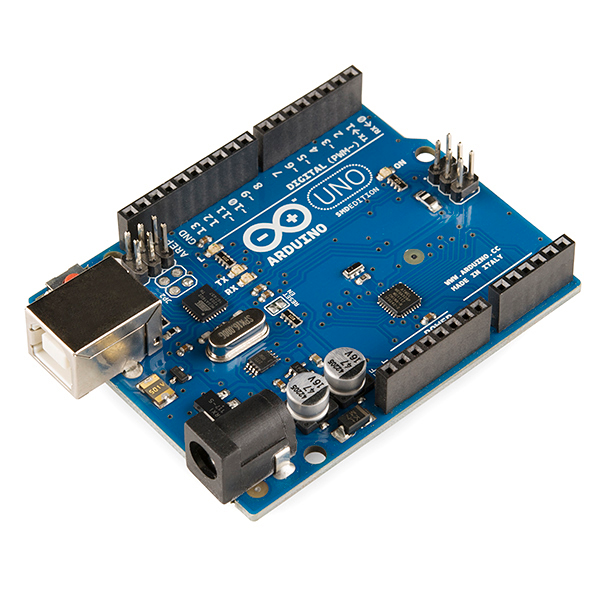
\includegraphics[width=.2\paperwidth]{images/arduino.png}}
	\end{center}
	\caption{ \textit{Une carte Arduino Uno}}
\end{figure}\\

	\item Installation du logiciel Arduino
	\item Découverte du logiciel et des bases de la programmation Arduino
	\item Mise en pratique
	\item Approfondissement
\end{itemize}\\

\section{Mise en pratique : Réalisation d'un feu tricolore}\\

\subsection{Objectifs}\\
\begin{enumerate}\\
	\item Monter un circuit sur BreadBoard permettant d'allumer / éteindre les LEDs grâce à l'Arduino
	\\
	\item Réaliser un petit programme reproduisant le comportement d'un feu tricolore
	\\
\end{enumerate}\\

\begin{figure}[H]
	\begin{center}
		\makebox[\textwidth]{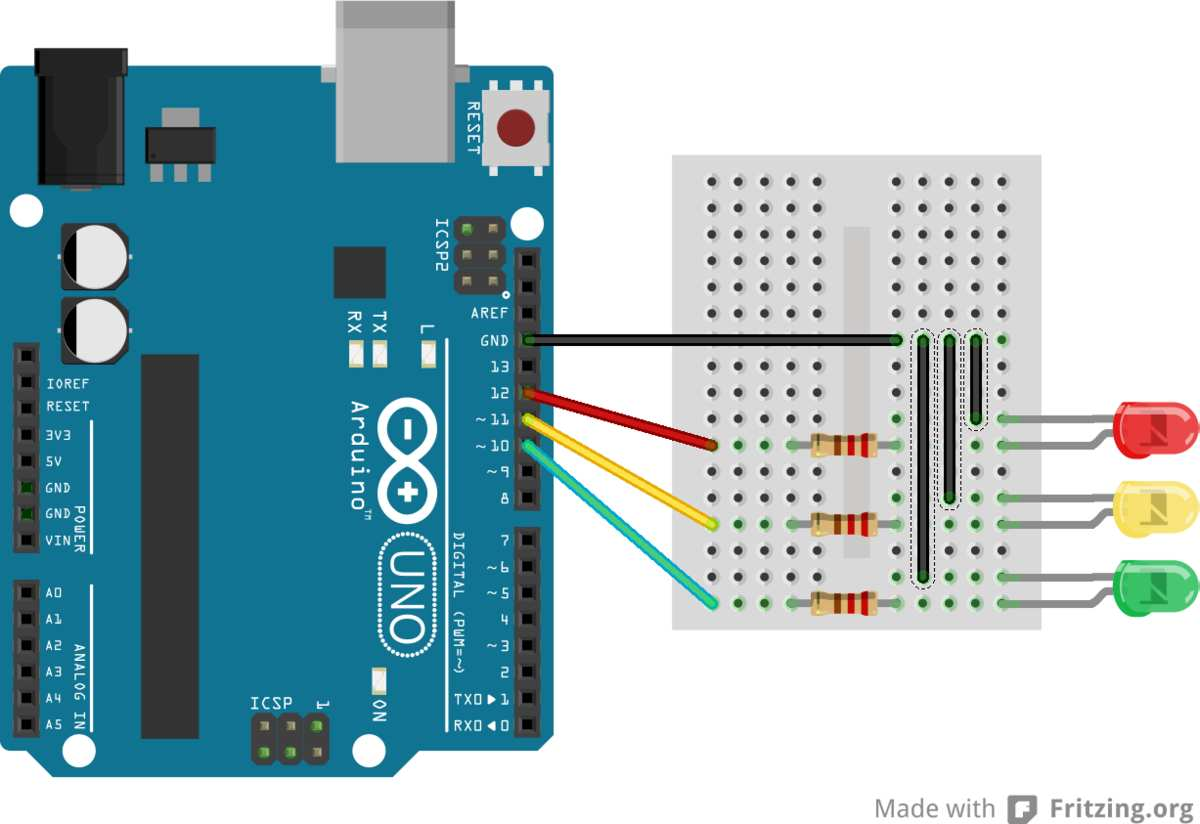
\includegraphics[width=.3\paperwidth]{images/montage1.png}}
	\end{center}
	\caption{ \textit{ Schéma de montage de l'Atelier 1}}
\end{figure}\\

\subsection{Approfondissement}\\

\begin{itemize}\\
	\item Réaliser un petit programme permettant d'utiliser le montage précédent pour compter en binaire.
\end{itemize}\\





%\input{./conclusion.tex}
\newpage
%\input{./annexe.tex}
\newpage
\nocite{*}

\end{document}